\section{Durchführung}
\label{sec:Durchführung}
Für diesen Versuch werden Ultraschallsonden mit einer Frequenz von $\qty{2}{\mega\hertz}$ verwendet,
die über einen Verstärker an einen Computer angeschlossen werden.
Am Computer werden mithilfe einer Software die Daten aufgenommen und graphisch dargestellt.
Die Sender bzw. Empfänger, sowie die Testkörper untereinander, werden bei jeder Messung mit bidestillierten Wasser oder
speziellem Gel gekoppelt.

\subsection{Verifizierung des Messverfahrens}

Zur Überprüfung des Messverfahrens sowie der Geräte und Software wird eine Acrylplatte verwendet.
Die Dicke der Acrylplatte wird gemessen und zu $10\,\unit{\milli\metre}$ bestimmt.
Es wird ein Scan mithilfe des \textit{Impuls-Echo-Verfahren} durchgeführt und das Ergebnis graphisch festgehalten.
Aus diesen Daten kann die Schallgeschwindigkeit und somit widerum die Dicke der Acrylplatte bestimmt werden.
Dieses experiementelle Ergebnis wird in \ref{sec:Verifizierung des Messverfahrens} ausgewertet
und mit den theoretischen Werten verglichen.

\subsection{Vermessung von Acrylzylindern}

Hier beginnt die Durchführung des eigentlichen Versuches, mit dem Ziel, die Geschwindigkeit sowie die Dämpfung
von Schallwellen in Acryl zu bestimmen.
Verwendet werden 4 Zylinder aus Acryl, deren Länge zuerst gemessen wird.
\begin{align*}
    \text{Zylinder 1:}\,l_1&=40,4\,\unit{\milli\metre} \\
    \text{Zylinder 2:}\,l_2&=61,5\,\unit{\milli\metre} \\
    \text{Zylinder 3:}\,l_3&=80,5\,\unit{\milli\metre} \\
    \text{Zylinder 4:}\,l_4&=120,5\,\unit{\milli\metre}
\end{align*}

Als erstes wird eine Sonde oben auf einem Zylinder platziert und die Laufzeit des Pulses mithilfe des \textit{Impuls-Echo-Verfahren}
gemessen. Dieses Vorgehen wird 6 mal wiederhohlt, dabei werden auch Zylinder kombiniert, um unterschiedliche Längen zu erhalten.

Danach wird wieder die Laufzeit gemessen, allerdings nach dem \textit{Durchschallungs-Verfahren} und für jedeglich die
vier einzelnen Zylinder.

Mithilfe der gewonnenen Daten wird in der Auswertung für beide Verfahren ein experimenteller Wert der Schallgeschwindigkeit bestimmt. \\

Zuletzt wird wieder die Messreihe des \textit{Durchschallungs-Verfahren} durchgeführt, diesmal werden anstatt der Laufzeiten die
Amplituden vor und nach der Reflektion am unteren Ende des Zylinders aufgenommen.
Aus deren Verhältnis wird in der Auswertung die Dämpfung der Schallwellen in Acryl berechnet.

\subsection{Vermessung eines Augenmodells}

Abschließend soll das Modell eines menschlichen Auges mithilfe des \textit{Impuls-Echo-Verfahren} vermessen werden.
Die Ultraschallsonde wird mithilfe des Gels an der Iris an das Auge gekoppelt und das Signal graphisch festgehalten.
Die Auswertung der Daten liefert dann Werte für die Abstände der verschiedenen Bestandtteile im Auge.
\begin{figure}
    \centering
    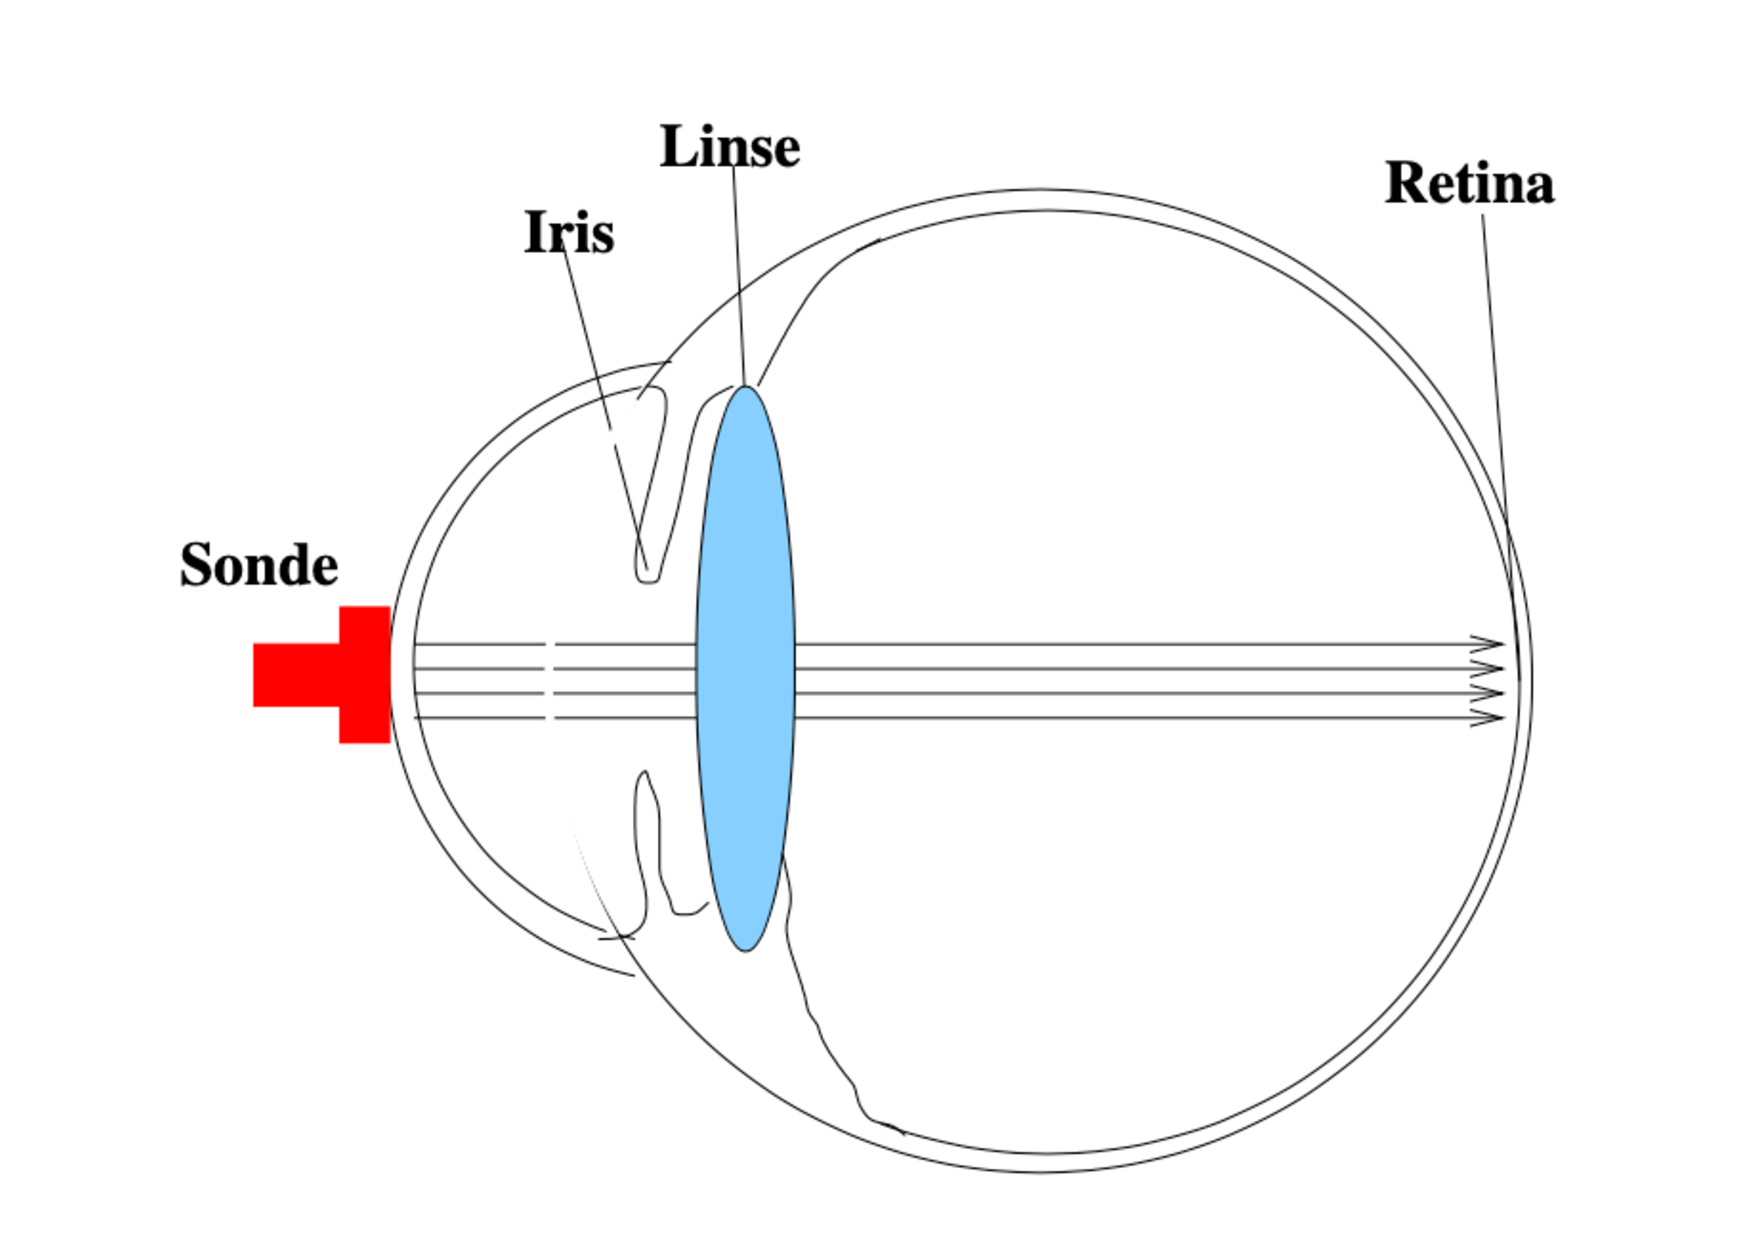
\includegraphics[height=6cm]{content/Abbildungen/Schema_Auge.pdf}
    \caption{Schema des menschlichen Auges.\cite{US1}}
    \label{fig:Schema Auge}
\end{figure}